\documentclass[12pt,a4paper]{article}
\usepackage[utf8]{inputenc}
\usepackage[a4paper]{geometry}
\usepackage{graphicx}
\usepackage{apacite}
\usepackage{float} % Put the images where they should be.

\begin{document}
\begin{titlepage}


\centering
  
  
{\scshape\LARGE Master thesis planning report\\}
  
\vspace{0.5cm}
  
{\huge\bfseries Enforcing Clients to Act Honestly in Verifiable Additive Homomorphic Secret Sharing\\}
  
\vspace{2cm}
  
{\Large Hanna Ek, hannakristinek@gmail.com\\}
  
\vspace{0.2cm}
  
  
\vspace{1.0cm}
  
{\large Supervisor at CSE: Georgia Tsaloli and Katerina Mitrokotsa\\}
  
\vspace{1.5cm}

  
\vspace{1.5cm}


  
\vspace{1.5cm}

\vfill

  

\vfill
  
{\large \today\\} 



\end{titlepage}
\pagenumbering{roman}
\newpage
\tableofcontents  
\newpage
\pagenumbering{arabic}
\setcounter{page}{1}
\section{Introduction}
This is a planning report for the master thesis of Hanna Ek during Spring $2021$. The thesis is supervised by Katerina Mitrokotsa professor at Chalmers and her phD student Gerogia Tsaloli. The preliminary title of this master project is \textit{Enforcing Clients to Act Honestly in Verifiable Additive Homomorphic Secret Sharing}.

\subsection{Background}
% Why is it relevant?
Digitalisation of the society leads to a need of cryptographic protocols to obtain online security and privacy. One privacy problem is when several parties wish to compute a joint output without their inputs being revealed. A concrete example could be extracting medical information about a group of people without leaking classified information about clients.

A cryptographic scheme for performing calculations on data from several clients without revealing individual information is additive homomorphic secret sharing. This protocol allows multiple clients to share information to one or several servers which then outputs the sum of the inputs, without leaking information about individual clients input. To ensure that the server(s) is not malicious and leaks information one can extend the protocol to include public verification of the output, i.e. anyone can verify that the servers' output is the correct sum of the inputs without knowing the input. This protocol is then named verifiable additive homomorphic secret sharing (VHASS). 

In an article published last year three different constructions for VHASS are presented, \cite{Georgia-orginal}. The constructions makes use of hash functions, linear homomorphic signatures and threshold signature sharing respectively to check that output is the correctly computed sum of the inputs. The protocols presented in \cite{Georgia-orginal} assumes that the clients are honest, i.e., the there is no check whether the clients input is correct or not. There are several applications of VHASS where the clients can be assumed to provide honest input, but in applications where this is not guaranteed it is needed to provide a check of the clients input. This cannot be done in a straightforward manner since the privacy of clients input cannot be compromised. This leads to the issue of checking that the input is correct without knowing the value of input. 

A possible method for ensuring the honesty of clients while maintaining privacy is \textit{range proofs}, \cite{RANGE} \cite{DRYNX}. Range proofs are used to verify and ensure that the input is in a certain allowed range. There exist multiple ranges proof protocols which are based on different properties and hence some might me more or less suitable to use in various situations. 

It would be of interest to construct a VHASS scheme that forces clients to be honest. If a VHASS construction checks the clients input it would widen the use of VHASS to applications where clients cannot be assumed to act honestly. A possible extension of a VHASS scheme to oblige correct input from clients is to include a range proof in the protocol. This project aims to investigate if such a combination of a VHASS construction and a range proof is an attractive method for verifying clients honesty.  

\subsection{Project Aim}
%What should be accomplished?
%Describe your contribution with respect to concepts, theory and technical goals. Ensure that the scientific and engineering challenges stand out so that the reader can easily recognize that you are planning to solve an advanced problem. 

The aim of this master thesis is to possibly extend the work presented in \cite{Georgia} such that the construction also insures that the clients are honest. 

This goal is split into the following sub-goals:
\begin{enumerate}
    \item Perform a literature review on verifiability for the client-sides in protocols for VHASS. Verifiability includes to confirm their input is correct and hence force them to act honestly.
    \item Do a second literature study of different range proofs: compare their performance and investigate their differences. 
    \item To be able to systematic compare range proofs a methodology for such comparison is to be developed and defined.
    \item Investigate lightweight zero knowledge proofs (ZK-proofs): compare their performance to range proofs and the possibility to implement a ZK-proof into a VHASS construction.
    \item Based on the literature studies, on VHASS constructions and ranges proofs investigate the possibility to extend of the VHASS constructions presented in \cite{Georgia} to include a range proof. Thereby the constructions would also enforce honesty of the clients. 
    \item It is not certain that the extension of VHASS to include a range proofs is an attractive way to insure clients honesty for VHASS constructions. If this is the case the goal will be to  describe and motivate why.
    
\end{enumerate}
The fifth sub-goal is mainly to propose and evaluate \textit{ways to go} in order to include a check of clients input to a VHASS construction and provide a theoretical proof of the new construction's  accuracy regarding security, correctness and verifiability of serves and clients. An attempt to implement the suggested approach will be made, if methodology of including ranges proofs in VHASS constructions is found and time is available.

\subsection{Limitations}
The main limitation to this project is time. The limited time leads to the limitation of only considering the first VHASS construction based on homomorphic secret sharing, \cite{Georgia}. This is to withing the time frame (hopefully) be able to both propose an extension to this construction to ensure honest clients and implement the approach. An implementation of the approach will provide important results about runtime performance. 
%. What should be left out and why?
%A limitation of this project is that only range proofs will be investigated as a possible extension to VHASS protocols. There are other possibilities of methods for ensuring clients honesty in VHASS constructions but here only range proofs will be considered. The reason for this is to keep the thesis coherent and investigate one possibility carefully instead of many carelessly based on the time frame given.

%A second limitation, as mentioned above, is that the aim of this project is to propose a method for testing clients input without trying to implement this method. An attempt to implement the suggested method will only be made if time is available. Please note that this possible implementation is not a part of the original goal of this project. 


\subsection{Ethical considerations}
The area of application for the results of this master thesis is in VHASS constructions in cryptography protocols. It is critical that in any such application the privacy of clients is not compromised. Hence the results presented must be carefully checked not to lead security loss when used in a cryptography protocol.  Since the application area is withing security and privacy the correctness and evaluation of results is particularly important for this thesis.


\section{Methodology}
% How should the work be carried out?
This section describes the methodology to fulfil the goals described above. The thesis will consist of large literature study to achieve a great understanding of client verification i VHASS constructions and range proofs. This will then be used to propose a possible extension to the work presented in \cite{Georgia-orginal} to insure honest clients.

\subsection{Literature study and investigation}
The first part of this master thesis will be to gather information. This will be done by literature studies and closer investigations of the studied areas. First about VHASS constructions and verifiability on the client-side and then about range proofs. Along with the literature study on range proofs a performance comparison between different range proofs will be made. This is to get an understanding of different range proofs advantages and disadvantages which will be useful in the next step of the thesis. To systematic compare and evaluate range proofs a methodology for performing such comparisons will be developed. A smaller literature study on lightweight ZK-proofs will also be carried out. Where there performance will be compared to range proofs.

\subsection{Combining VHASS construction and range proofs}
After the two literature studies the next step will be to try to extend the VHASS constructions presented in \cite{Georgia-orginal} with a check of the clients input. This will be done by exploring the possibilities to combine VHASS constructions with a range proof. The range proof will be applied to the clients input. The work on including a range proof to a VHASS construction will be done by testing different range proofs and evaluate the security, computational effort and simplicity for each. A model for systematic comparison will be developed to insure a scientific and fair judgement.

If a satisfying extension is found, the next step will be to prove its performance. This implies to prove that the proposed method forces clients to act honestly in the VHASS protocol and prove that the security, correctness and verification of the original VHASS construction has not been compromised. Then the complexity of the new construction will be determined.

If time is available an code implementation of the suggested approach will be made and runtime measurements will be carried out. 

If it is found that including a range proof to a VHASS construction is not
an attractive way to insure clients honesty, the work will instead be to explain why.

\section{Time plan}
The master thesis will be performed between the weeks $3$ and $22$ in $2021$. A Gantt schedule for the project is seen in Figure \ref{fig:Gantt}. The goal is to follow this time schedule but the work is flexible to change if parts turnout to take longer or shorter time. All mandatory element and deadlines of the thesis work is included in the Gantt schedule and marked with red dots. 
\begin{figure}[]
\centering
    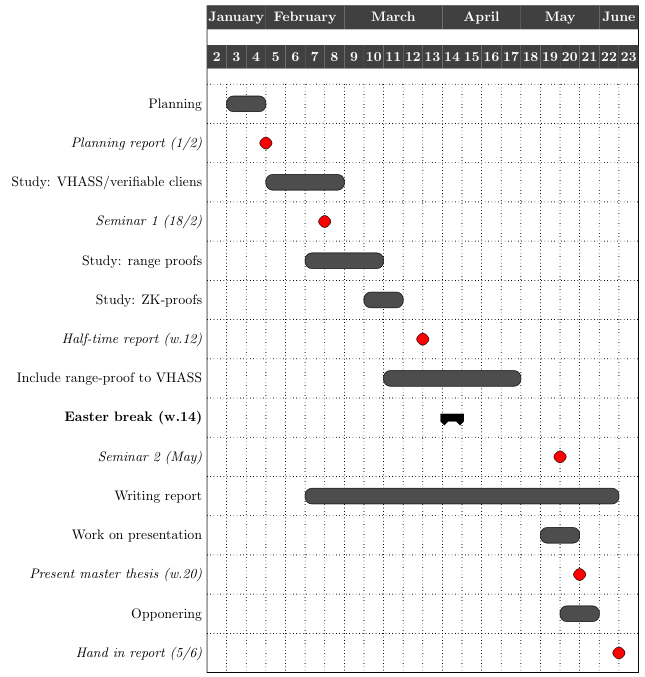
\includegraphics[width=1.1\linewidth]{gantt.png}
    \caption{Gantt scheme for this master thesis}
    \label{fig:Gantt}
\end{figure}
\newpage


\bibliographystyle{apacite}
\bibliography{bibliography.bib}


\end{document}
